\documentclass[11pt,letterpaper]{article}
\usepackage[utf8]{inputenx} %Codificacion del texto (ISO Latin1 encoding)

\usepackage{fancyhdr} %Permite acomodar a tu gusto la parte de arriba y
% abajo del documento
\usepackage[spanish]{babel} %Permite definir el idioma del dcumento
\usepackage{graphicx} %Permite exportar imagenes en formato eps
\usepackage{url} %Tipo de fuente para correos y paginas
\usepackage{pgf}
\usepackage{fleqn}
\usepackage{amssymb}
\usepackage{amsmath}
\usepackage{bigints}
\usepackage{fancyvrb}
\usepackage{makeidx}
\usepackage{colortbl} %Permite colocar colores a las tablas
\usepackage{multirow}
\usepackage{booktabs}
\usepackage{moreverb}
\usepackage{rotating}
\usepackage{lastpage}
\usepackage[final]{pdfpages}
%%%%%%%%%%
%Margenes%
%%%%%%%%%%
\usepackage[top=3cm,bottom=3cm,left=3cm,right=3cm,footskip=1.5cm,headheight=1.5cm,headsep=.5cm,textheight=3cm]{geometry}
%%%%%%%%%%%%%%%%%%%%%%
%Estilo del documento%
%%%%%%%%%%%%%%%%%%%%%%
\pagestyle{fancyplain}

%%%%%%%%%%%%%%%%%%%%%%%%%%%%%%%%%%%%%%%%%%%
%Fancyheadings. Top y Bottom del documento%
%%%%%%%%%%%%%%%%%%%%%%%%%%%%%%%%%%%%%%%%%%%
% Recuerde que en este documento la portada del documento no posee
% numeracion, pero de igual manera llamaremos a esa primera pagina la numero
% 1, y la que viene la dos. Esto es para tener una idea de las que
% llamaremos pares e impares
\lhead{Laboratorio mat024} %Parte superior izquierda
\rhead{\bf \it Preinforme 3} %Parte superior derecha
\lfoot{\it Victor Gonzalez} %Parte inferior izquierda. \thepage indica
% el numero de pagina
\cfoot{\bf \thepage} %Parte inferior central
\rfoot{página \thepage\ de \pageref{LastPage}} %Parte inferior derecha
\renewcommand{\footrulewidth}{0.4pt} %Linea de separacion inferior

\begin{document}
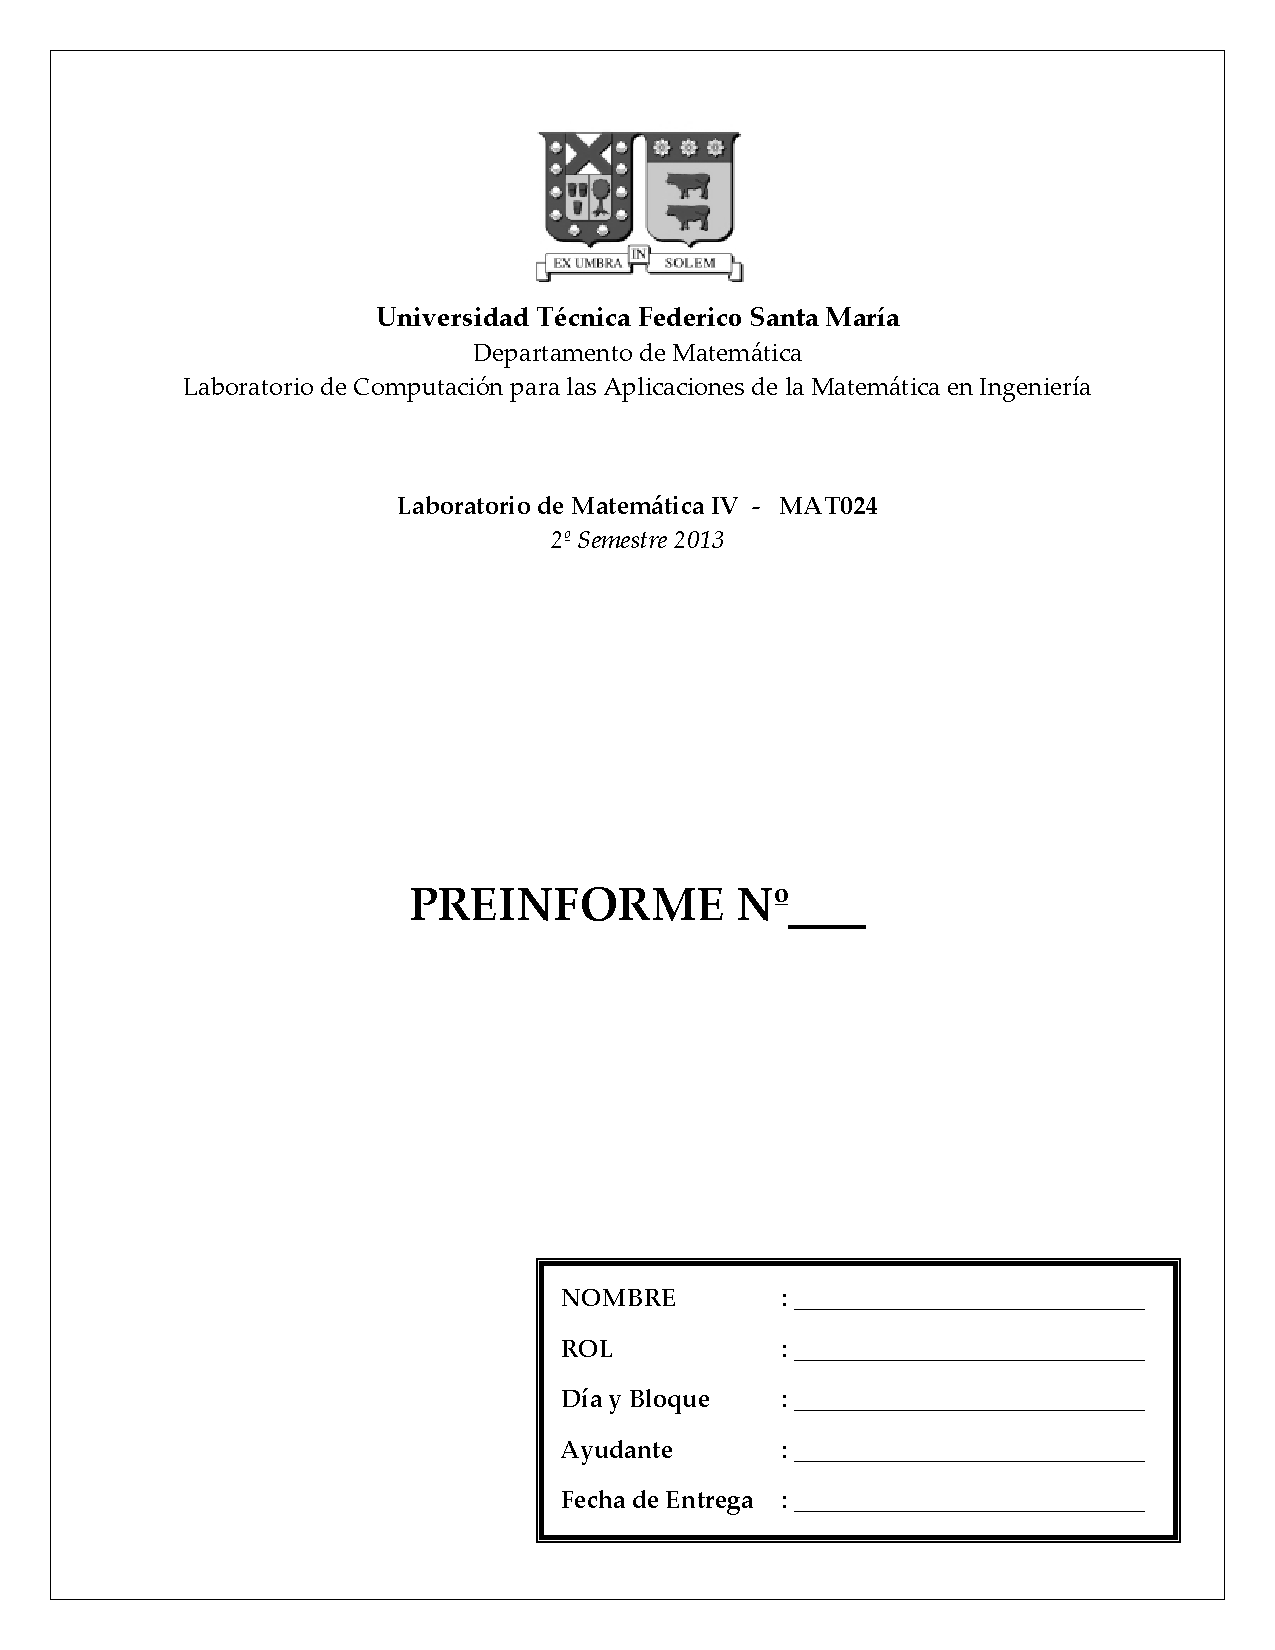
\includepdf[pages={1}]{portada.pdf}

\section{Desarrollo Analítico y Planteamiento}
\subsection{Pregunta 1}

Se nos pide calcular el flujo que pasar por la intersección de 3 superficies, las cuales definiremos como:

\begin{center}$S_1: x^2+y^2+z^2=4$\end{center}
\begin{center}$S_2: z+2=0$\end{center}
\begin{center}$S_3: x^2+y^2=z-1$\end{center}

Y además existe un campo vectorial $\vec{F}=\{x^3,y^3,z^3\}$. Luego, la gráfica la podemos observar en el anexo, donde se aprecia la superficie encerrada por $S_1$, $S_2$ y $S_3$, junto con el campo vectorial.

Para simplificar el cálculo, trabajaremos con coordenadas esféricas, las cuales vienen dadas por $t=\{x,y,z\}$, donde:

\begin{center}$x=2Cos(\theta)Sin(\phi)$\end{center}
\begin{center}$y=2Sin(\theta)Sin(\phi)$\end{center}
\begin{center}$z=2Cos(\phi)$\end{center}

Ahora, buscamos encontrar el flujo mediante Gauss, el cual viene dado por: $\bigointss_\Gamma \vec{F}\vec{n}ds$.

El vector normal $\vec{n}$, se calcula utilizando el producto cruz entre las derivadas parciales de la parametrización. Luego, $\vec{n}=t_\theta$x$t_\phi$, el cual es $\vec{n}=$\noindent\(\left\{4 \text{Cos}^2(\theta ) \text{Sin}^2(\phi),4 \text{Sin}^2(\theta ) \text{Sin}^2(\phi),2 \text{Sin}(2 \phi )\right\}\).

Por otro lado, al aplicar la transformación sobre $\vec{F}$, obtenemos que\\ $\vec{F}=$ \noindent\(\left\{8 \text{Cos}^3(\theta) \text{Sin}^3(\phi ),8 \text{Sin}^3(\theta ) \text{Sin}^3(\phi),8 \text{Cos}^3(\phi)\right\}\).
\\

Solamente nos queda encontrar los parámetros de integración. Para ello, observamos la gráfica y notamos que el parámetro $\theta$ recorre su rango completo, es decir $0\leq \theta \leq 2\pi$. Pero el parámetro $\phi$, recorre desde la intersección entre $S_1$ con $S_3$, hasta su rango máximo, el cual es $\pi$.

Finalmente, utilizando \textit{Mathematica}, calculamos ese límite de integración.

Luego, la integral de Gauss queda como:

\begin{center}
$\bigointss_\Gamma \vec{F}\vec{n}ds=\bigintss_0^{2\pi}\bigintss_{0.86}^\pi \vec{F}\vec{n}d\phi d\theta = 199.331$\end{center}

Por lo tanto, el flujo que pasa a través de la superficie encerrada entre $S_1,S_2$ y $S_3$ es $199.331$.
\subsection{Pregunta 2}
Utilizamos $u(r,\theta) = v(r,\theta)+\phi(theta)$ donde $\phi(\theta)$ tiene que ser escogido de manera que obtengamos un problema homogéneo. Para ello, $\phi(\theta)$ debe satisfacer:

\begin{center}$\phi''(\theta)=2$,    $\phi(0)=0$,$\phi(\pi)=\pi^2$\end{center}

Luego, es sencillo ver que la solución para esa ecuación es $\phi(\theta)=\theta^2$. Por lo tanto, el problema homogeneo queda como:
\begin{center}
\begin{tabular}{r c l l l}
$r^2v_{rr}+rv_r+v_{\phi\phi}$ & $=$ & $0$ & $0 < r < +\infty$, &  $0 < \phi < \pi$ \\
$v(r,0)$ & $=$ & $0$ & $0 < r < +\infty$, & \\
$v(r,\pi)$ & $=$ & $0$ & $0 < r < +\infty$, &  \\
$v_r(a,\theta)$ & $=$ & $f(\theta)$ & $0 < r < \pi$, &   \\
\end{tabular}
\end{center}

La solución se puede obtener mediante separación de variables utilizando $v(r,\phi)=m(r)n(\phi)$, obteniendose:

\begin{center}
$\dfrac{r^3m''+rm'}{-m}=\dfrac{n''}{n}=-\lambda$
\end{center}

Podemos observar que tenemos una igualdad muy conveniente. Al utilizarla, nos encontramos con la siguiente ecuación:

\begin{center}
\begin{tabular}{r c l l }
$n''+\lambda n$ & $=$ & $0$ & $0 < r < \pi$\\
$n(0)$ & $=$ & $n(\pi)=0$ &  \\
\end{tabular}
\end{center}

Por otro lado, tenemos el problema en variable $r$, el cual al despejarse, se observa que es una \textit{ecuación de Euler}: $r^3m'' + rm' -\lambda m = 0$.

Pero del problema de \textit{Sturm-Liouville}, se sabe que uno de los valores propios asociados es $\lambda_k = -k^2$ y su función propia asociada es $\sigma_k(\phi)=Sin(k\phi)$. Luego, acotando mediante las condiciones dadas, obtenemos que la solución a la EDP es:

\begin{center}
$u(r,\theta)=\sum\limits_{k=1}^\infty \sigma_k r^{-\lambda_k}Sin(k\phi )$
\end{center}


\section{Conclusiones}
Gracias al teorema de Gauss, es posible hacer calculos sobre superficies complejas de una manera muy sencilla, las cuales usandose apropiadamente, aceleran mucho los cálculos.

Mientras que para las ecuaciones diferenciales parciales, tenemos herramientas muy variadas, las cuales permiten resolver mas mecánicamente, ecuaciones complejas, mediante simples teoremas ya demostrados y que se pueden ocupar directamente.

\includepdf[pages={1,2}]{lab3_mathematica.pdf}

\end{document}